%
%
%
We ran several problems with an fixed number of grid points in the problem's volume, varying $n$ and $\ell$ proportionally, \emph{i.e.}, $\bar{n} = n \times \ell$ for some fixed $\ell$.
Each hybridized system has more than 705\,600 points as the $\textbf{F}$  factors increase the size of the system as we add elements.
Each problem was run with several thread configurations, from 1 thread to 28 threads. 
Additionally total number of elements varied between 9, with 78\,400 grid points per element and 1600, with 441 grid points per elements. 
With this we have a profile of the problem's strong-scaling performance, as well as an insight in the effects of varying element size within the same problem.  

%
%
%
The optimal runtime was found at $\ell^2 = 100$ for all thread configurations. 
A full table of the compute time separated by thread count and element count is given in \figref{fig:tts_total}.
We plot the speedup \emph{i.e.}, $S = T/T_{p}$ for the number of threads $p$ for the best and worst choices of $\ell$ in \figref{fig:sca_exp_a}.

%
%
%
\begin{figure}[h]
	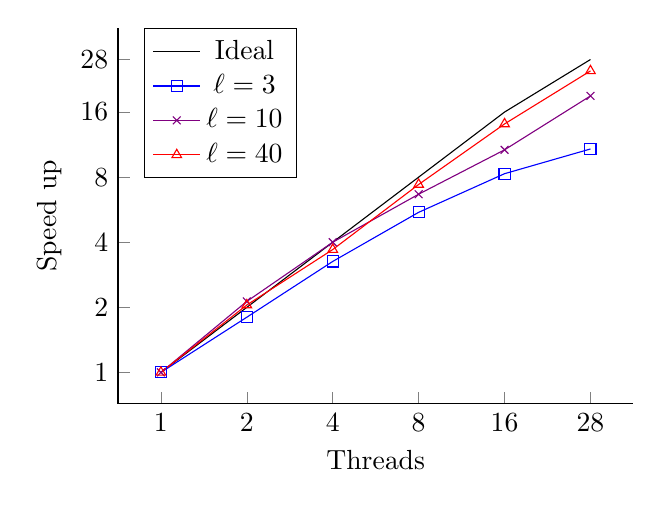
\begin{tikzpicture}
    \begin{axis}[
        legend style = {
            at={(0.05, 1)},
            anchor = north west,
            legend columns = 1},
        height=2.5in,
        width=3.2in,
        axis x line*=bottom,
        axis y line*=left,
        symbolic x coords = {1, 2, 4, 8, 16, 28},
        xtick = {1, 2, 4, 8, 16, 28},
        ytick = {1, 2, 4, 8, 16, 28},
        domain = 1:28,
        range = 1:28,
        ymode = log,
        log ticks with fixed point,
        xlabel={Threads},
        ylabel={Speed up}]      
        \addplot[
            no markers,
            color=black] coordinates {
                (1, 1)
                (2, 2)
                (4, 4)
                (8, 8)
                (16, 16)
                (28, 28)
            };                 
        \addplot[
            mark=square,
            color=blue] coordinates {
                (1, 1)
                (2, 1.8)
                (4, 3.26)
                (8, 5.5)
                (16, 8.3)
                (28, 10.8)
            };
        \addplot[
            mark=x,
            color=violet] coordinates {
                (1, 1)
                (2, 2.13)
                (4, 4)
                (8, 6.67)
                (16, 10.7)
                (28, 19)
            };
        \addplot[
            mark=triangle,
            color=red] coordinates {
                (1, 1)
                (2, 2.05)
                (4, 3.7)
                (8, 7.4)
                (16, 14.1)
                (28, 24.8)
            };
        \addlegendentry{Ideal}
        \addlegendentry{$\ell = 3$}
        \addlegendentry{$\ell = 10$}
        \addlegendentry{$\ell = 40$}
    \end{axis}
\end{tikzpicture}
	\caption{
	    The speed up of three pairs of $n$ and $\ell$ such that $\bar{n}$ is constant. 
	    Scaling improves as $\ell$ increases; however, overall runtime is best at $ell = 10$. 
	    }
    \label{fig:sca_exp_a}
\end{figure}

Here, speedup scaling is proportional to $\ell$. 
This is not in proportion to the overall runtime by choice of $\ell$; the best case ($\ell^2 = 100$) has worse scaling than $\ell^2 = 1600$ and better than $\ell^2 = 9$.
This suggests that different components of the problem are contributing to the performance on either end of of this scale. 

%
%
%
To this end we profiled the runtime of the 7 operations that comprise the hybridized system. 
Two operations utilize the majority of the compute time, those being SpMV from \eqnref{eqn:global_system_b} and MatMul from \eqnref{eqn:global_system_a}.
The remaining 5 operations average $8\%$ of the compute time when run on a single thread. 
The compute time of the two major operations are plotted in \figref{fig:runtime_comps} with the same configuration of problems. 

%
%
%
\begin{figure}
\centering
\begin{subfigure}[b]{1\columnwidth}
\centering
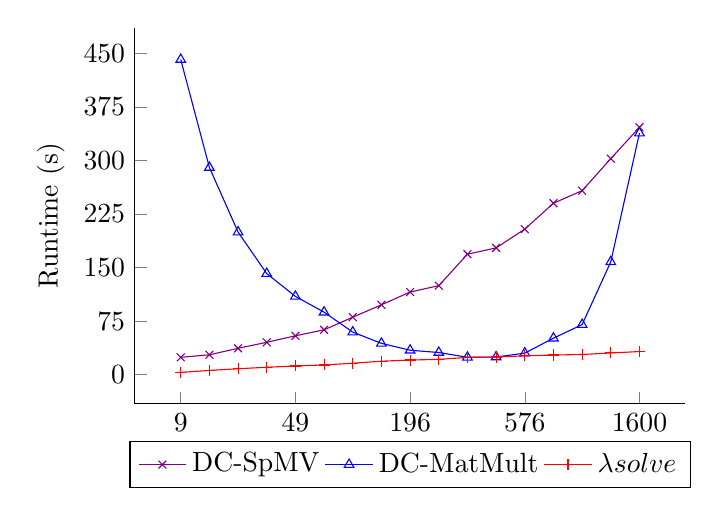
\begin{tikzpicture}
    \begin{axis}[
        legend style={
            at={(0.5,-0.1)},
            anchor=north,legend columns=-1},
        height=2.5in,
        width=3.375in,
        axis x line*=bottom,
        axis y line*=left,
        symbolic x coords = {9, 16, 25, 36, 49, 64, 100, 144, 196, 225, 400, 441, 576, 784, 900, 1225, 1600},
        xtick = {9, 49, 196, 576, 1600},
        ytick distance=75,
        domain = 9:1600,
        range = 0:450,
        xlabel={Elements},
        ylabel={Runtime (s)}]
        \addplot[
            mark=x,
            color=violet] coordinates {
                (9, 24.325156)
            	(16, 27.834308) 
            	(25, 36.956056)
            	(36, 45.347331)
            	(49, 54.437361)
            	(64, 62.814148)
            	(100, 80.488467)
            	(144, 97.845769)             	 
            	(196, 115.743751) 
            	(225, 124.628909) 
            	(400, 168.691478) 
            	(441, 177.584231) 
            	(576, 203.812683) 
            	(784, 240.088173) 
            	(900, 257.634123) 
            	(1225, 302.521926)
            	(1600, 346.441605)		
            };                
        \addplot[
            mark=triangle,
            color=blue] coordinates {
                (9, 441.321048)
            	(16, 290.10575)
            	(25, 199.676772)
            	(36, 141.542836)
            	(49, 109.624197)
            	(64, 87.516978)
            	(100, 59.597739)
            	(144, 43.86835)             	 
            	(196, 34.223977) 
            	(225, 31.043727) 
            	(400, 24.364813) 
            	(441, 24.756918) 
            	(576, 30.185676) 
            	(784, 51.117228) 
            	(900, 70.110809) 
            	(1225, 158.006306)
            	(1600, 338.225247)		
            };
        \addplot[
            mark=+,
            color=red] coordinates {
                (9, 3.186158)
            	(16, 5.987428)
            	(25, 8.304203)
            	(36, 10.420171)
            	(49, 12.213909)
            	(64, 13.637598)
            	(100, 16.047212)
            	(144, 18.873235)             	 
            	(196, 20.515413) 
            	(225, 21.414372)
            	(400, 24.244844) 
            	(441, 24.780033) 
            	(576, 26.379761) 
            	(784, 27.517695) 
            	(900, 28.265589) 
            	(1225, 30.447891)
            	(1600, 32.383344)		
            };
        \addlegendentry{DC-SpMV}
        \addlegendentry{DC-MatMult}
        \addlegendentry{$\symbf{\lambda} \text{ solve}$} 
    \end{axis}
\end{tikzpicture}
\end{subfigure}
\begin{subfigure}[b]{1\columnwidth}
\centering
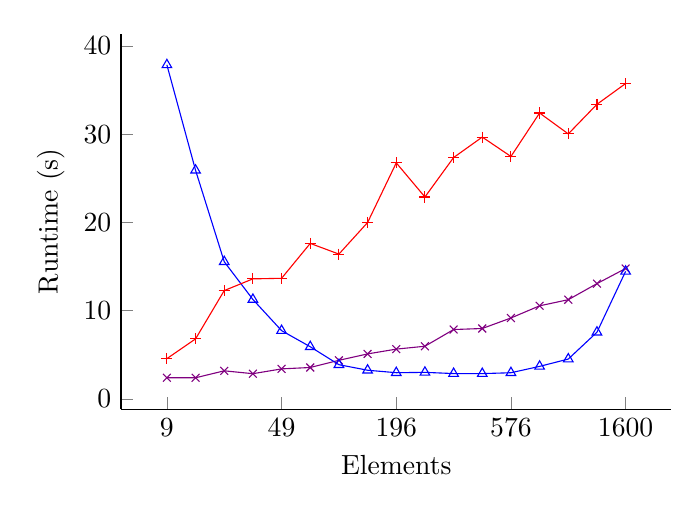
\begin{tikzpicture}
    \begin{axis}[
        height=2.5in,
        width=3.375in,
        axis x line*=bottom,
        axis y line*=left,
        symbolic x coords = {9, 16, 25, 36, 49, 64, 100, 144, 196, 225, 400, 441, 576, 784, 900, 1225, 1600},
        xtick = {9, 49, 196, 576, 1600},
        ytick distance=10,
        domain = 9:1600,
        range = 0:40,
        xlabel={Elements},
        ylabel={Runtime (s)}]
        \addplot[
            mark=x,
            color=violet] coordinates {
                (9, 2.397702)
                (16, 2.394517) 
                (25, 3.180994)
                (36, 2.855465)
                (49, 3.40153)
                (64, 3.558418)
                (100, 4.372501)
                (144, 5.095191)                  
                (196, 5.641578) 
                (225, 5.964769) 
                (400, 7.857667) 
                (441, 7.976037) 
                (576, 9.166833) 
                (784, 10.545802) 
                (900, 11.238055) 
                (1225, 13.058728)
                (1600, 14.773929)       
            };                            
        \addplot[
            mark=triangle,
            color=blue] coordinates {
                (9, 37.839475)
                (16, 25.899214)
                (25, 15.539969)
                (36, 11.263805)
                (49, 7.735455)
                (64, 5.908895)
                (100, 3.875921)
                (144, 3.248426)                  
                (196, 2.967249) 
                (225, 3.007436) 
                (400, 2.871237) 
                (441, 2.866318) 
                (576, 2.963138) 
                (784, 3.684828) 
                (900, 4.5139599) 
                (1225, 7.553876)
                (1600, 14.450906)       
            };     
        \addplot[
            mark=+,
            color=red] coordinates {
                (9, 4.562236)
                (16, 6.799783)
                (25, 12.272318)
                (36, 13.599193)
                (49, 13.662346)
                (64, 17.617201)
                (100, 16.404489)
                (144, 19.981687)                 
                (196, 26.740117) 
                (225, 22.875268)
                (400, 27.343023) 
                (441, 29.659641) 
                (576, 27.462272) 
                (784, 32.388184) 
                (900, 30.020221) 
                (1225, 33.37332)
                (1600, 35.725706)       
            };

    \end{axis}
\end{tikzpicture}
\end{subfigure}
\caption{Runtime of routines that significantly contribute to the overall
    runtime for various element configurations. 1 thread (top) and 28 
    threads (bottom). }
\end{figure}

%
%
%
We exclude the time spent factorizing $\textbf{M}$ and $\symbf{\lambda}_{\textbf{A}}$ for this problem, its practical application would likely involve the reuse of these factorization several times. 
It is worth noting that the cost of LU factorization for $\symbf{\lambda}_{\textbf{A}}$ becomes considerable as $\ell^2$ increases. 
This is expected by \eqnref{eqn:lamsize} as the size of $\symbf{\lambda}_{\textbf{A}}$ increases with $\ell$ and by \eqnref{eqn:nz_sum} as the number of non-zeros increases with $\ell$.

%
%
%
\subsection{MatMul analysis}

%
%
%
\begin{figure}
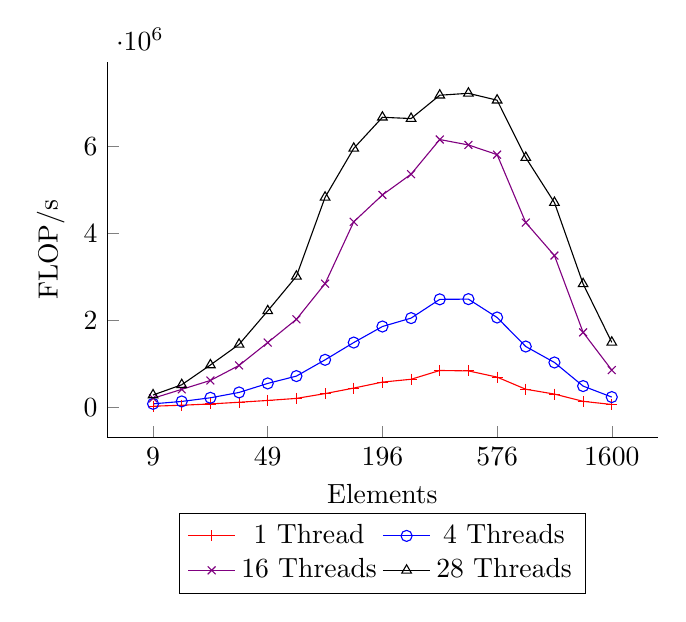
\begin{tikzpicture}
    \begin{axis}[
	    legend style={
            at={(0.5,-0.2)},
            anchor=north,
            legend columns=2},
        height=2.5in,
        width=3.375in,
        axis x line*=bottom,
        axis y line*=left,
        symbolic x coords = {9, 16, 25, 36, 49, 64, 100, 144, 196, 225, 400, 441, 576, 784, 900, 1225, 1600},
        xtick = {9, 49, 196, 576, 1600},
        ytick distance=2000000,
        domain = 9:1600,
        range = 0:10000000,
        xlabel={Elements},
        ylabel={FLOP/s}]
	\addplot[
        mark=+,
        color=red] coordinates {
            (9,24160.18916)
			(16,46212.11403)
			(25,75762.76323)
			(36,115210.3523)
			(49,156578.57)
			(64,203576.4992)
			(100,314453.8084)
			(144,441429.8691)
			(196,578962.5209)
			(225,644095.8587)
			(400,846784.4182)
			(441,837067.0372)
			(576,694117.3025)
			(784,414388.6676)
			(900,303442.8543)
			(1225,135813.9212)
			(1600,63858.08331)};
	\addlegendentry{1 Thread}
    \addplot[
        mark=o,
        color=blue] coordinates {
            (9,78513.66238)
			(16,133745.4278)
			(25,217815.5867)
			(36,340888.9967)
			(49,548515.3324)
			(64,717364.6669)
			(100,1091864.432)
			(144,1489948.304)
			(196,1859190.77)
			(225,2052879.643)
			(400,2484952.613)
			(441,2489810.713)
			(576,2067020.621)
			(784,1398554.858)
			(900,1030993.746)
			(1225,487411.0526)
			(1600,234183.1179)};
	\addlegendentry{4 Threads}
	\addplot[
        mark=x,
        color=violet] coordinates {
            (9, 206894.3049)
			(16, 412005.2777)
			(25, 616785.9578)
			(36, 963066.0121)
			(49, 1490017.073)
			(64, 2024705.029)
			(100, 2846381.623)
			(144, 4270917.234)
			(196, 4889061.938)
			(225, 5368039.349)
			(400, 6165113.665)
			(441, 6040768.307)
			(576, 5817354.332)
			(784, 4252592.221)
			(900, 3493402.238)
			(1225, 1724497.681)
			(1600, 855346.1252)};
	\addlegendentry{16 Threads}
	\addplot[
        mark=triangle,
        color=black] coordinates {
            (9,281779.808)
			(16,517637.3306)
			(25,973493.8339)
			(36,1447752.336)
			(49,2218977.423)
			(64,3015183.042)
			(100,4835169.757)
			(144,5961287.097)
			(196,6677700.456)
			(225,6648565.755)
			(400,7185663.879)
			(441,7229902.614)
			(576,7071017.28)
			(784,5748545.115)
			(900,4713074.266)
			(1225,2840853.623)
			(1600,1494606.359)};
	\addlegendentry{28 Threads}
    \end{axis}
\end{tikzpicture}
\caption{Performance of the decomposed MatMult kernel on a fixed problem size (705600 grid points) for various thread counts and total elements.}
\end{figure}
										
													


%
%
%
Out of the two kernels that comprise the majority of the runtime we see the most variability in MatMul operation from \eqnref{eqn:global_system_a}. 
The operation is implemented in a similar manner to batched general matrix multiply (GEMM) methods \citep{wei2022lbbgemm}, but as our intermediate results from $\textbf{M}^{-1}\textbf{F}$ are dense vectors we instead compute a batched vector inner product. Batching methods allocate single threads to self-contained operations in contrast to  of coordinating multiple threads to solve a larger problem. 

These results show an optimal range of elements to minimize runtime between 100 to 600 elements for $\bar{n} = 840$.
When there are too few elements the problem has a greater number of FLOPs and bytes loaded. 
The total FLOPs of this operation decrease for MatMul at a rate of $1/\ell^4$ from \eqnref{eqn:flops_fmf} and the total bytes decrease at $1/\ell^3$ from \eqnref{eqn:bytes_fmf}.
As both of these terms decrease, our runtime decreases proportionally until we reach approximately 600 elements. 

%The increase in runtime at this point is associated with increasing number of non-zeros in $\symbf{\lambda}_{\textbf{A}}$. 

\begin{figure}
	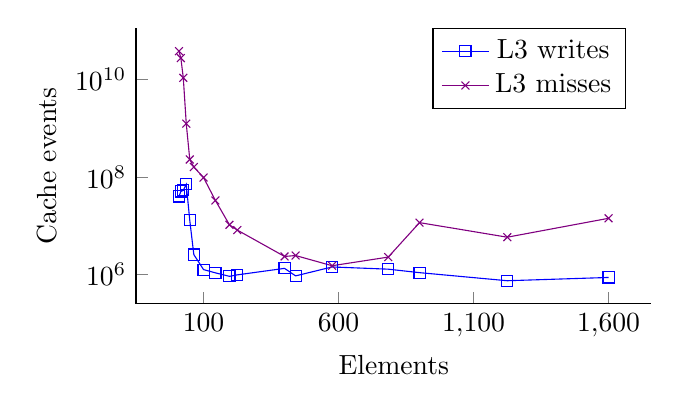
\begin{tikzpicture}
    \begin{axis}[
        legend style = {
            at={(0.95, 1)},
            anchor = north east,
            legend columns = 1},
        height=2in,
        width=3.2in,
        axis x line*=bottom,
        axis y line*=left,
        xtick={100, 600, 1100, 1600},
        domain = 1:1600,
        range = 1:1e10,
        ymode = log,
        xlabel={Elements},
        ylabel={Cache events}]                     
        \addplot[
            mark=square,
            color=blue] coordinates {
                (9,40205717)
                (16,50879473)
                (25,53610700)
                (36,71074406)
                (49,12977133)
                (64,2579077)
                (100,1268591)
                (144,1087212)
                (196,922253)
                (225,988667)
                (400,1344455)
                (441,941907)
                (576,1436403)
                (784,1294177)
                (900,1097877)
                (1225,749441)
                (1600,874811)
            };
        \addplot[
            mark=x,
            color=violet] coordinates {
                (9,38402769309)
                (16,27712437645)
                (25,10922310284)
                (36,1249621355)
                (49,230572757)
                (64,161468223)
                (100,98065404)
                (144,33179551)
                (196,10523799)
                (225,8202903)
                (400,2360980)
                (441,2462776)
                (576,1522457)
                (784,2288844)
                (900,11663667)
                (1225,5858703)
                (1600,14307506)
            };
        \addlegendentry{L3 writes}
        \addlegendentry{L3 misses}
    \end{axis}
\end{tikzpicture} 
	\caption{L3 writes and misses profiled for the strong scaling problem configuration. 
	Though the total bytes written out to $\symbf{\lambda}_{\textbf{A}}$ increase with additional elements, fewer occur with every batch. 
	Fewer writes per batch to more rows of $\symbf{\lambda}_{\textbf{A}}$ increase our cache misses and overall runtime.
	}
	\label{fig:mmwm}
\end{figure}

%but writes increase with the rate of non-zeros in $\symbf{\lambda}_{\textbf{A}}$ in \eqnref{eqn:nz_sum}. 

%As each element becomes smaller and we increase the number of iterations, the number of writes per iteration decrease. 



%This CPU is rated at a peak single-threaded FLOP rate of 8 GFLOPS/s and a peak memory bandwidth of 86 GB/s.


%From this figure we see that the MatMul operation has a region of optimal performance between 196--576 elements, but begins to perform poorly outside of this range. 
%This is clear as \fig
